\documentclass[12pt]{beamer}
\usetheme{Malmoe}
\usepackage[utf8]{inputenc}
\usepackage{graphicx}
\usepackage{xcolor}
\usepackage{wrapfig} % texlive-latex-extra package

\definecolor{Cyan}{RGB}{0,141,184}
\setbeamercolor{structure}{fg=Cyan}

\author{Ivan Minčík}
\title{GIS.lab}
\subtitle{rapid GIS office deployment}
%\setbeamercovered{transparent} 
%\setbeamertemplate{navigation symbols}{} 
%\logo{} 
%\institute{} 
%\date{} 
%\subject{} 
\begin{document}

\begin{frame}
	\titlepage
\end{frame}


\section{Task}
\begin{frame}{What does it take to build a small GIS office?}
	\textbf{Conditions}
	\begin{itemize}
		\item 12 people staff with equipment
		\item Server and client hardware
		\item No software installed
		\item All hardware connected to LAN
	\end{itemize}
\end{frame}


\begin{frame}{What does it take to build a small GIS office?}
	\textbf{Requirements}
	\begin{itemize}[<+->]
		\item Office suite
		\item Desktop GIS software for technical staff (data processing, analysis)
		\item Web GIS software for non-technical staff (map browsing, queries)
		\item Central file data storage and sharing
		\item Central GIS vector and raster data storage and sharing
		\item Collaboration tools
		\item Central backup
		\item Quick hardware failure recovery
	\end{itemize}
\end{frame}


\begin{frame}
	\LARGE \textbf{How to do it ?}
\end{frame}


\section{Solutions}
\subsection{Legacy system}
\begin{frame}{Legacy system}
	\textbf{Server}
	\begin{itemize}[<+->]
		\item Server operating system
		\item Central authentication
		\item Internet connection (DNS, proxy)
		\item File storage and sharing
		\item Email
		\item Geo-database
		\item Mapserver (WMS, WFS)
		\item Web GIS application
		\item Backup and recovery
	\end{itemize}
\end{frame}


\begin{frame}{Legacy system}
	\textbf{Workstations}
	\begin{itemize}[<+->]
		\item Desktop operating system (Win 8 or Win 7?)
		\item Security
		\item User account
		\item Desktop environment customization
		\item Office suite
		\item Email, chat
		\item GIS software
	\end{itemize}
\end{frame}


\begin{frame}{Legacy system}
	\begin{flushleft}
		\textbf{\textcolor{Cyan}{?} days, weeks, months} \\
		\textbf{\textcolor{Cyan}{?} EUR} \\
	\end{flushleft}
\end{frame}


\begin{frame}
	\LARGE \textbf{Anything better?}
\end{frame}


\subsection{GIS.lab}
\begin{frame}{GIS.lab}
	One command to install server and clients
	\begin{flushleft}
		\textbf{\textcolor{Cyan}{20} minutes} \\
		\textbf{\textcolor{Cyan}{0} EUR} \\
	\end{flushleft}
\end{frame}


\subsection{GIS.lab Unit}
\begin{frame}{GIS.lab Unit}
	\begin{minipage}[\textheight]{\textwidth}
	\begin{columns}[T]
		\begin{column}{0.5\textwidth}
			\vspace{0.2\textheight}
			Plug-and-play
			\begin{flushleft}
				\textbf{\textcolor{Cyan}{0} minutes} \\
				\textbf{\textcolor{Cyan}{450} EUR} \\
			\end{flushleft}
		\end{column}
		\begin{column}{0.5\textwidth}
			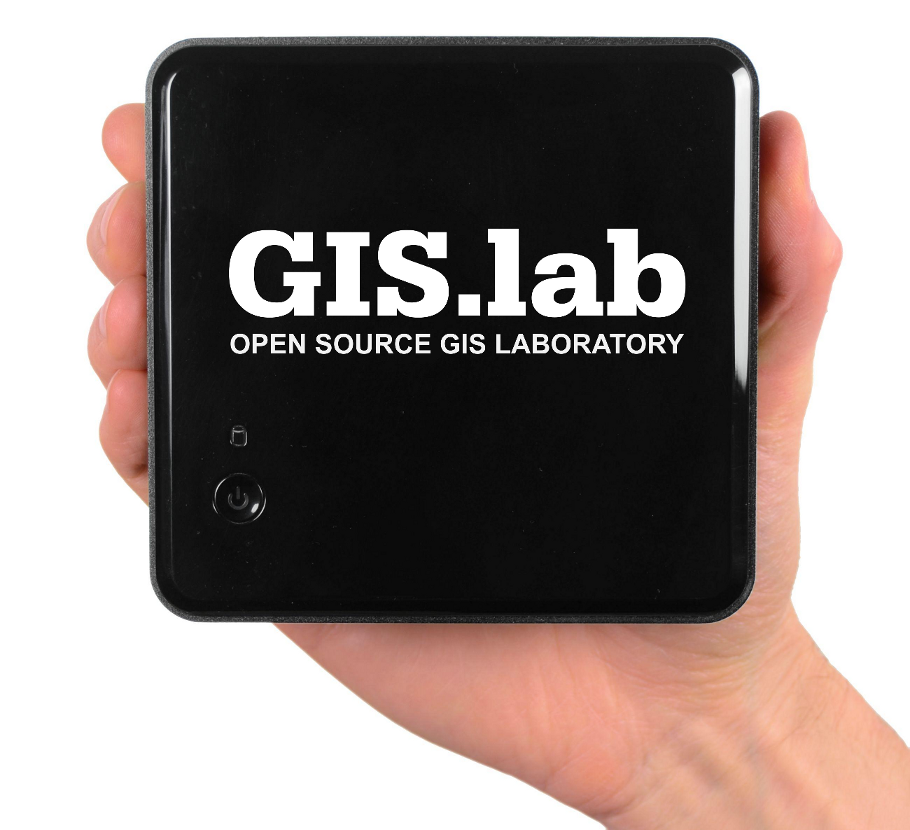
\includegraphics[keepaspectratio=true,width=\textwidth]{images/gislab-unit.png}
		\end{column}
	\end{columns}
	\end{minipage}
\end{frame}


\begin{frame}
	\LARGE \textbf{How it works?}
\end{frame}

\section{How GIS.lab works}
\subsection{Architecture}
\begin{frame}{GIS.lab architecture}
	\begin{center}
		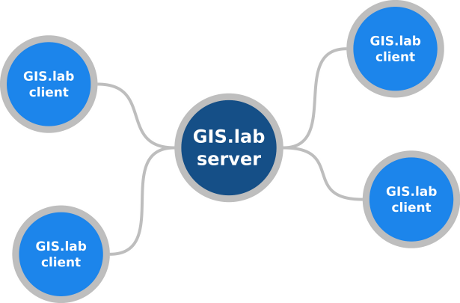
\includegraphics[keepaspectratio=true,height=0.4\textheight]{images/gislab-architecture.png}
	\end{center}
	\begin{columns}
		\begin{column}{0.5\textwidth}
			\textbf{GIS.lab server}
			\begin{itemize}
				\item automatic provisioning (Win, Lin, Mac)
				\item network boot service
				\item other services and data
			\end{itemize}				
    	\end{column}
		\begin{column}{0.5\textwidth}
			\textbf{GIS.lab client}
			\begin{itemize}
				\item boot from network
				\item mount system and data
				\item high performance, minimal server load
			\end{itemize}
		\end{column}
	\end{columns}	
\end{frame}


\subsection{Physical client}
\begin{frame}{Physical client}
	\begin{center}
		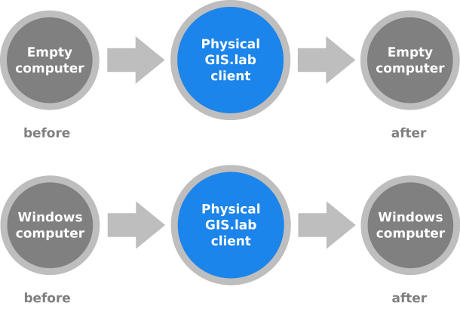
\includegraphics[keepaspectratio=true,height=0.5\textheight]{images/schema-physical-client.png}
	\end{center}
	\begin{columns}
		\begin{column}{0.5\textwidth}
			\begin{itemize}
				\item original OS isn't accessible 
			\end{itemize}				
    	\end{column}
		\begin{column}{0.5\textwidth}
			\begin{itemize}
				\item best performance
			\end{itemize}
		\end{column}
	\end{columns}	
\end{frame}


\subsection{Virtual client}
\begin{frame}{Virtual client}
	\begin{center}
		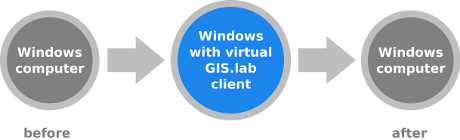
\includegraphics[keepaspectratio=true,height=0.3\textheight]{images/schema-virtual-client.png}
	\end{center}
	\begin{columns}
		\begin{column}{0.5\textwidth}
			\begin{itemize}
				\item original OS and GIS.lab client runs side-by-side 
			\end{itemize}				
    	\end{column}
		\begin{column}{0.5\textwidth}
			\begin{itemize}
				\item windowed or full screen mode
			\end{itemize}
		\end{column}
	\end{columns}	
\end{frame}


\subsection{Features and benefits}
\begin{frame}{Features and benefits}
	\begin{itemize}
		\item Open Source software (GNU GPL 3)
		\item Plug-and-play solution GIS.lab Unit
		\item No hard dependency on any other Internet service (with exception on OSM and Google maps)
		\item General usage platform (not limited to GIS)
	\end{itemize}
\end{frame}


\begin{frame}{Features and benefits}
	\begin{itemize}
		\item Extremely low maintenance costs
		\begin{itemize}
			\item zero time to install new client machine
			\item central distribution of client systems with rollback
			\item rapid recovery from hardware failure
		\end{itemize}
		\item High performance client systems (opposite of thin client)
	\end{itemize}
\end{frame}


\begin{frame}{Features and benefits}
	\textbf{Server services}
	\begin{itemize}
		\item Internet connection sharing
		\item Central authentication
		\item File storage and sharing
		\item Central data backup and recovery
	\end{itemize}
\end{frame}


\begin{frame}{Features and benefits}
	\textbf{Office suite}
	\begin{itemize}
		\item Text documents, tables and presentations processor
		\item Internet browser
		\item Email and chat client
		\item Images and video viewer and editor
	\end{itemize}
\end{frame}


\begin{frame}{Features and benefits}
	\textbf{GIS features}
	\begin{itemize}
		\item OpenStreetMap, Google base maps
		\item GIS data editor (desktop and web)
		\item GIS analysis tools
		\item Print composer
		\item GIS data storage and sharing (geo-database)
		\item OWS services (WMS, WFS)
		\item Instant export to WebGIS application from all GIS projects
	\end{itemize}
\end{frame}


\subsection{Utilization}
\begin{frame}{Utilization}
	\begin{itemize}
		\item Desktop environment for small GIS businesses
		\item Education
		\item Crisis Mapping
		\item GIS software development environment
		\item Parallel computing
	\end{itemize}
\end{frame}


\section{Example work flow}
\begin{frame}{Example work flow}
	Task: xxxx
\end{frame}


\begin{frame}{Example work flow}
	TODO: Screenshots
\end{frame}


\section{About}
\begin{frame}{About}
	\begin{itemize}
		\item Authors: Ivan Minčík, Marcel Dancák
		\item Sponsor: GISTA s.r.o. www.gista.sk
		\item Partner: University of Prešov in Prešov, www.unipo.sk
		\item Development state: in active development
		\item Credits: developers of Linux, Debian, Ubuntu, Xubuntu, VirtualBox, Vagrant, LTSP, PostgreSQL, PostGIS, PgAdmin, SpatiaLite, QGIS, GRASS GIS, Django, GeoExt, OpenLayers and tons of other Open Source software
		\item Home page: \textbf{http://imincik.github.io/gis-lab}
		\item License of this presentation: CC BY-SA
	\end{itemize}
\end{frame}


\begin{frame}{Used technologies - server}
	\textbf{Host machine requirements}
	\begin{itemize}
		\item Operating System - Linux or Windows or Mac OS X
		\item Virtualization software - VirtualBox or VMWare or LXC containers
		\item Provisioning software - Vagrant
	\end{itemize}

	\textbf{Software and Services}
	\begin{itemize}
		\item Boot from LAN tool chain - TFTP, DHCP, LTSP
		\item DNS - BIND
		\item File sharing - NFS
		\item Database - PostgreSQL/PostGIS
		\item Mapping server and web GIS - Apache, QGIS Mapserver, GIS.lab WebGIS
		\item Chatting server - IRC
	\end{itemize}	
\end{frame}


\begin{frame}{Used technologies - client}
	\textbf{Host machine requirements}
	\begin{itemize}
		\item Nothing or
		\item Operating System Linux or Windows or Mac OS X
	\end{itemize}

	\textbf{Software and Services}
	\begin{itemize}
		\item Office suite - LibreOffice, Firefox, Thunderbird, Pidgin, GIMP, VLC ...
		\item GIS software - QGIS, GRASS, Spatialite, PgAdmin
		\item Developer tools - Git, QtCreator, Python, GIS libraries
	\end{itemize}	
\end{frame}


% document END
\end{document}